\documentclass[11pt, oneside]{article}   	% use "amsart" instead of "article" for AMSLaTeX format
\usepackage{geometry}                		% See geometry.pdf to learn the layout options. There are lots.
\geometry{letterpaper}                   		% ... or a4paper or a5paper or ... 
%\geometry{landscape}                		% Activate for for rotated page geometry
%\usepackage[parfill]{parskip}    		% Activate to begin paragraphs with an empty line rather than an indent
\usepackage{graphicx}				% Use pdf, png, jpg, or eps� with pdflatex; use eps in DVI mode
								% TeX will automatically convert eps --> pdf in pdflatex		
\usepackage{amssymb}
\usepackage{amsmath}
\usepackage{parskip}
\usepackage{color}
\usepackage{hyperref}

\title{Gaussian integral by volume and more}
%\author{The Author}
%\section{}
%\subsection*{}
\date{}							% Activate to display a given date or no date

\graphicspath{{/Users/telliott_admin/Dropbox/Tex/png/}}
% \begin{center} 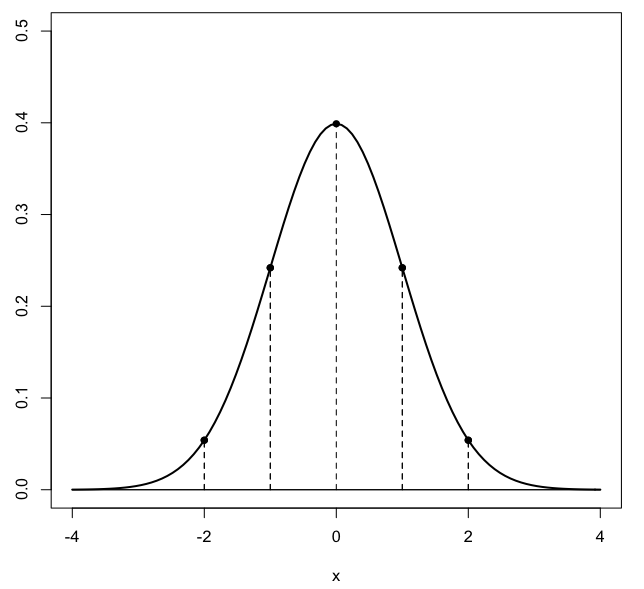
\includegraphics [scale=0.4] {gauss3.png} \end{center}
\begin{document}
\maketitle
\large
We wish to solve this integral:
\[ I = \int_{-\infty}^{\infty} e^{-x^2/2} \ dx \]
The solution is:
\[ I = \sqrt{2 \pi} \]

We will prove this using a method based on integrating volumes.

\url{http://www.math.uconn.edu/~kconrad/blurbs/analysis/gaussianintegral.pdf}

Consider the "bell surface" or Gaussian surface formed by the (unnormalized) function, lacking any corrective factor in front of the exponential.  For this section we will take $V=1$.
\[ z = e^{-(x^2 + y^2)/2} \]

It looks like this:
\begin{center} 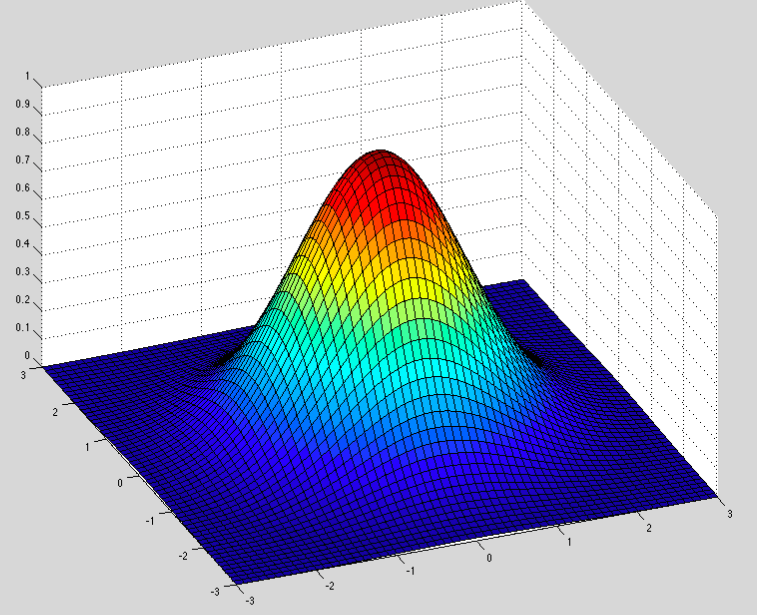
\includegraphics [scale=0.4] {gaussian-surface.png} \end{center}
It's a real bell!

We compute the volume under the surface in two ways.  The first way is by horizontal slices perpendicular to the $z$-axis.

\subsection*{Horizontal}
\[ \int_0^b A(z) \ dz \]
We need an expression for the area of horizontal slices as a function of the height $z$.  What we have now is the inverse function:
\[ z = e^{-(x^2 + y^2)/2} \]
So let's do it:
\[ x^2 + y^2 = -2 \ \ln z \]
The horizontal cross-sections (at $z = c$, where $c$ is a constant), are circles of radius $r$: where
\[ r^2 = x^2 + y^2 = -2 \ \ln z \]

We will fix the upper bound as follows:  the maximum value of $z$ occurs when $x=y=0$ and the exponential is equal to $1$, otherwise the value is less than $1$, so we have that 
\[  z = e^{-(x^2 + y^2)/2} = e^0 = 1 \]
This will be the upper bound on $z$ when we calculate the volume.

So finally, the integral we need starts with $A = \pi r^2$:
\[ A(z) = \pi \ (-2) \ \ln z \]
\[ V = -2 \pi \int_0^1 \ln z \ dz \]
    
Now (leaving the factor of $-2 \pi$ aside for now) that is just:
\[ \int \ln z \ dz = z \ln z - z \]
which is easily verified by differentiating the result.

We need to evaluate this expression between the bounds we set above ($z=0 \rightarrow 1$).

At the lower bound of $z=0$, clearly the second term is zero.
  
The first term is $\ \ln z$.  To evaluate:
\[ \lim_{z \rightarrow 0+}  z \ \ln z  \]

we use L'Hopital's rule:  
\[ z \ \ln z = \frac{z}{1/\ln z} \]

As $z \rightarrow 0+$, the numerator is just zero and the denominator is :$1/-\infty = 0$ so by the rule, we compute the derivatives:
\[ \frac{1}{1/(1/z)} = z \]
And this limit is equal to zero so we have just zero for the whole expression at the lower bound.

At the upper bound, the first term is zero and the second is equal to $-1$.

Remembering the extra factor, we have finally just $(-2 \pi)(-1) = 2 \pi$.

\subsection*{Vertical}

The other way is vertical slices.  First, recall our definition:
\[ I = \int_{-\infty}^{\infty} e^{-x^2/2} \ dx \]

Again, $I$ is what we're looking for.  It is \textbf{just a number}.  So
\[ z = e^{-(x^2 + y^2)/2} \]
If we take slices perpendicular to the $x$-axis (with $x =$ constant for any particular slice), the area of each slice is
\[ A(x) = \int_{-\infty}^{\infty} e^{-(x^2 + y^2)/2} \ dy \]
since  $x$ is a constant we have
\[ = e^{-x^2/2} \ \int_{-\infty}^{\infty} e^{-y^2/2} \ dy = e^{-x^2/2} \ I \]

Now we add up all the little slices to find the volume, which is
\[  V =  \int_{-\infty}^{\infty} I e^{-x^2/2} \ dx \]
but $I$ is just a number, so
\[  =  I \int_{-\infty}^{\infty} e^{-x^2/2} \ dx \]
\[ = I^2 \]

Now we have two different expressions for the same volume, which must be equal to each other.  Thus:
\[ 2 \pi = I^2 \]
\[ I = \sqrt{2 \pi} \]

\subsection*{Gamma function}

The Gamma function is:
\[  \Gamma(x) = \int_0^{\infty} t^{x-1} e^{-t} \ dt \]

A bit more about it here:

\url{https://en.wikipedia.org/wiki/Gamma_function}

For integer $n$
\[  \Gamma(n) = (n-1)! \]
Here is one important property of the gamma function that is easily proved using integration by parts:
\[ \Gamma (x+1) = x \Gamma(x) \]
The gamma function is like the factorial, but it generalizes to non-integer values of $x$, and it's offset by $1$.

A second property that I got from the reference above, but have to investigate in more detail is:
\[ \frac{\Gamma(x) \Gamma(y)}{\Gamma (x+y)} = \int_0^1 t^{x-1}(1-t)^{y-1} \ dt \]

\subsection*{Trick with x = 1/2}
In any case, using this last equation, set
\[  x = y = \frac{1}{2} \]
then
\[ [ \ \Gamma(\frac{1}{2}) \ ]^2 = \int_0^1 \frac{1}{\sqrt{t(1-t)}} \ dt \]
Now, from the standard gamma function definition:
\[ \Gamma(x) = \int_0^{\infty} t^{x-1} e^{-t} \ dt \]
\[ \Gamma(\frac{1}{2}) = \int_0^{\infty} \frac{1}{\sqrt{t}} e^{-t} \ dt \]
Substitute $\sqrt{t} = x$, so then $t = x^2$ and $dt = 2 x \ dx$, and
\[ \Gamma(\frac{1}{2}) = \int_0^{\infty} \frac{1}{x} e^{-x^2} \ 2 x \ dx \]
\[ = 2 \int_0^{\infty} e^{-x^2} \ dx \]

\subsection*{Defining J}
This integral is related to what we called $I$ before.  

Recall:
\[ I = \int_{-\infty}^{\infty} e^{-x^2/2} \ dx \]
Two differences are the bounds on the integral and the factor of $1/2$ in the exponent.  

Define 
\[ J = \int_{-\infty}^{\infty} e^{-x^2} \ dx \]
And since $J$ is an even function, we have that
\[ J = 2 \int_{0}^{\infty} e^{-x^2} \ dx \]
which is exactly what we had above.  Therefore:
\[ \Gamma(\frac{1}{2}) = J \]
\[ [ \ \Gamma(\frac{1}{2}) \ ]^2 = J^2 \]
So then
\[ J^2 = \int_0^1 \frac{1}{\sqrt{t(1-t)}} \ dt \]

\subsection*{Second integral}
To do this last integral, substitute:
\[  t = \sin^2 \theta \]
\[  dt = 2 \sin \theta \cos \theta \ d \theta \]
\[ \sqrt{t(1-t)} = \sqrt{t} \ \sqrt{1-t} = \sin \theta \cos \theta \]
So the integral is simply $2 \theta$ (!!!)  What are the bounds?
\[ t = 0 \Rightarrow \sin^2 \theta = 0 \Rightarrow \theta = 0 \]
\[  t = 1 \Rightarrow \sin^2 \theta = 1 \Rightarrow \theta = \frac{\pi}{2} \]
    The final value is just $\pi$.  So:
\[ J^2 = \int_0^1 \frac{1}{\sqrt{t(1-t)}} \ dt = \pi \]
 \[ J = \sqrt{\pi} \]

\subsection*{Relating I and J}
To finish up, we need to determine the relationship between:
\[  I = \int_{-\infty}^{\infty} e^{-x^2/2} \ dx \]
and
\[ J = \int_{-\infty}^{\infty} e^{-x^2} \ dx \]
We just do a simple substitution:
\[ u = \frac{x}{\sqrt{2}} \]
\[ \sqrt{2} \ du = dx \]
\[ I = \int_{-\infty}^{\infty} e^{-u^2} \ \sqrt{2} \ du \]
\[ = \sqrt{2} \ J \]
Hence:
\[ I = \sqrt{2} \ J = \sqrt{2} \ \sqrt{\pi} = \sqrt{2 \pi} \]

Note:  in the reference they define $J$ as the integral from $0 \rightarrow \infty$.  Since $J$ is also an even function, this $J$ is twice theirs.

\end{document}  